% ============================================================
%  CHAPTER 3 — PROPOSED SYSTEM ARCHITECTURE
%  Corrected 2026-08-28 -- see VERIFICATION_NOTES.md.
%  Every numeric/technical claim below was checked against either
%  CLAUDE.md's verified state or, where noted, the live source file
%  directly (backend/llm/llm_client.py, backend/agents/validation_agent.py).
%  Where a specific implementation detail (exact FSM field list, frontend
%  component names, HNSW parameters) was NOT independently re-verified in
%  this pass, it is marked %% VERIFY AGAINST CODE rather than stated as
%  fact -- do not remove that marker without actually checking the file
%  named in the comment.
% ============================================================
\chapter{Proposed System Architecture}
\label{chap:architecture}

This chapter presents the architecture of the multilingual conversational AI
system for Labour Force Survey administration, sourced directly from the
live implementation rather than restated from an earlier, unverified draft.

% ------------------------------------------------------------
\section{Design Principles}
\label{sec:arch-principles}
% ------------------------------------------------------------

\textbf{P1 --- Transparency and auditability.}
Every ISCO-08 classification carries a method label (e.g.\ flat retrieval,
hierarchical retrieval, keyword fallback, LLM fallback) so a result is never
silently reported as one method when another actually produced it. When
ISCO, ISIC, and ISCED data are all available, a \texttt{semantic\_coherence}
object is included in the survey message response.

\textbf{P2 --- Standards compliance.}
Classifications reference ISCO-08 (ILO,
2012)~\cite{ilo2012isco_v1,ilo2012isco_v2} and ISCED~2011 / ISCED-F~2013
(UNESCO UIS)~\cite{unesco2012isced}.
%% VERIFICATION NEEDED: the original draft cited zhou2025llmdata (an
%% unrelated LLM/data-management survey paper) as the source for ISIC
%% Rev.4 -- that citation was clearly wrong and has been removed here.
%% No correct ISIC Rev.4 UNSD citation exists in bib.bib yet; add one
%% (UNSD, "International Standard Industrial Classification of All
%% Economic Activities, Revision 4", 2008) before submission.
Qdrant collections are versioned by profile name (see
Section~\ref{sec:arch-rag}) rather than mutated in place --- a new profile
(e.g.\ \texttt{official\_ilo2021\_v1\_enriched\_e5large}) is built and
verified independently before any production switch, and multiple profiles
coexist live.

\textbf{P3 --- Privacy-aware design.}
Email OTP + JWT authentication, with \texttt{sendgrid==6.12.5} and
\texttt{python-jose[cryptography]==3.5.0} confirmed as real, pinned
dependencies in \texttt{requirements.txt} --- both genuinely used, not
carried over unchecked from an earlier draft. Per-row PII access logging
exists in the \texttt{data\_access\_logs} table (see
Chapter~\ref{chap:implementation}).
%% VERIFICATION NEEDED: the exact OTP/audit-log retention period (e.g.
%% "10 years") was not independently re-verified against the live code in
%% this pass.

\textbf{P4 --- Calibrated uncertainty and HITL escalation.}
\texttt{ISCOClassifier.HITL\_THRESHOLD = 0.70}: composite confidence below
this triggers escalation. LLM re-ranking is skipped when top-1 similarity is
$\geq 0.92$ (a real, confirmed fast-path threshold --- see
Chapter~\ref{chap:evaluation}'s discussion of how often this path actually
fires: 99.7\% of a real 18,747-case run fell \emph{below} 0.92, meaning the
LLM step fires on nearly every real query, not the exception this design
might suggest). \texttt{HITLQualityManager} maintains its own, separately-set
thresholds (\texttt{\_LOW\_CONFIDENCE\_THRESHOLD=0.60},
\texttt{\_MIN\_PASS\_QUALITY\_SCORE=0.70}, \texttt{\_ESCALATION\_THRESHOLD=0.50}) ---
stated here as genuinely independent of \texttt{ISCOClassifier}'s own
threshold, not unified into one number, because that is how the live code is
actually structured.

\textbf{P5 --- Deterministic response-consistency validation.}
The \texttt{ValidationAgent} enforces ten deterministic rules, R01--R10,
verified directly against \texttt{backend/agents/validation\_agent.py}:
required-field presence (R01), \texttt{hours\_per\_week} parseability (R02)
and range [1,168] (R03), an outlier warning above 80 hours/week (R04),
job-title/hours contradictions for unemployed (R05, R06) and
not-in-labour-force (R07) respondents, full-time/part-time hours-mismatch
warnings (R08, R09), and a zero-hours contradiction for employed respondents
(R10). \textbf{This corrects an earlier internal draft of this thesis},
which described R01--R10 as ILO ICLS-19-specific rules named ``E1'' (a wage
gate) and ``F3'' (a not-in-labour-force re-routing rule) --- neither of
those rule IDs or that specific behaviour exists in the real
\texttt{ValidationAgent}; the real ten rules are the hours/employment-status
consistency checks listed above.

\textbf{P6 --- Modularity.}
A Dockerised multi-service stack (backend, frontend, PostgreSQL, Qdrant,
Redis, Ollama). Agent modules under \texttt{backend/agents/} are invoked
directly by the API route handlers in \texttt{backend/api/survey\_routes.py}
--- there is no separate orchestrator module and no CrewAI hierarchical
delegation process anywhere in this codebase.

% ------------------------------------------------------------
\section{High-Level System Architecture}
\label{sec:arch-overview}
% ------------------------------------------------------------

The system has four logical layers.

\textbf{User Interface Layer.}
A Next.js~14 frontend confirmed to have four pages: \texttt{/} (home,
\texttt{index.js}), \texttt{/chat}, \texttt{/report}, and
\texttt{/supervisor\_review} (plus Next.js's own framework files
\texttt{\_app.js}/\texttt{\_document.js}), all confirmed loading against
the live system. \texttt{components/LanguageToggle.js} and
\texttt{components/api.js} are confirmed real, existing exactly as an
earlier internal draft of this thesis named them.
%% VERIFY AGAINST CODE: exact field/quick-reply counts ("39 categorical
%% fields") and RTL/font implementation details were not re-verified in
%% this pass.

\textbf{FastAPI Backend Layer.}
13 modules under \texttt{backend/agents/} each construct a
\texttt{crewai.Agent} (verified directly, all with
\texttt{allow\_delegation=False}): \texttt{audit\_logger},
\texttt{context\_memory}, \texttt{conversation\_manager},
\texttt{emotional\_intelligence}, \texttt{hitl\_quality\_manager},
\texttt{isco\_classifier}, \texttt{isic\_classifier},
\texttt{isced\_classifier}, \texttt{language\_processor}, \texttt{rag\_expert},
\texttt{report\_generator}, \texttt{semantic\_relation}, and
\texttt{validation\_agent}. Three further modules (\texttt{nationality\_
classifier}, \texttt{person\_register}, \texttt{isco\_reranker\_strict}) are
real, used modules that do \emph{not} construct a \texttt{crewai.Agent} ---
included here because an earlier internal draft of this thesis incorrectly
counted \texttt{person\_register} as one of its numbered agents. The system
exposes 20 distinct API routes (counted from the live OpenAPI specification;
see Chapter~\ref{chap:implementation}), not a single message endpoint.

\textbf{Knowledge and Data Layer.}
ISCO-08 retrieval is served from a real, verified 436-unit-group catalogue
(matching the official ILO count exactly, after a primary-source correction
--- see Section~\ref{sec:arch-rag}), indexed across \emph{multiple}
coexisting Qdrant collection profiles, not a fixed set of four: a legacy
profile, an official-ILO-source profile, e5-large and enriched-text
variants, and flat-retrieval variants (43 live collections confirmed via a
direct API call as of the most recent count in CLAUDE.md). ISIC Rev.~4 and
ISCED-F classifiers now have both a legacy keyword pipeline and real,
live Qdrant-backed hierarchical and flat retrieval paths (Section
\ref{sec:arch-isic}). PostgreSQL stores survey data across 11 tables (see
Chapter~\ref{chap:implementation}). Redis provides session context.

\textbf{LLM Routing Layer.}
\texttt{backend/llm/llm\_client.py} implements a \texttt{TaskType} enum with
exactly two values, confirmed directly from the live source:
\texttt{GENERAL} (Ollama/Llama~3.2, temperature~0.3, with an automatic
fallback chain --- Ollama~$\to$~Claude~$\to$~Gemini~$\to$~Groq~$\to$~
OpenRouter --- stopping at the first configured, reachable provider) and
\texttt{CRITICAL} (Claude~3.5~Sonnet, temperature~0.0, \textbf{with no
fallback at all} --- a deliberate design choice to pin a single
high-accuracy model for critical tasks, confirmed directly in the function's
own docstring). \textbf{A real, disclosed operational limitation}: this
project's Anthropic account has had zero usable credit throughout its
evaluation history (documented repeatedly in this project's own working
notes), so \texttt{TaskType.CRITICAL} calls have not been demonstrated to
succeed end-to-end against real Claude inference in this project's own
evaluation runs; where LLM re-ranking was actually measured (see
Chapter~\ref{chap:evaluation}), Groq and Gemini were used as substitutes,
never presented as Claude results.
\texttt{get\_llm\_strict()}, used by everything the evaluation harness
measures, never substitutes providers silently regardless of the above.

% ── System Architecture Diagram ─────────────────────────────
% ============================================================
%  System Architecture Diagram — corrected 2026-08-28
%  Rebuilt against verified facts: 13 real agent-constructing modules
%  (not 10), no CrewAI hierarchical process (removed -- none exists in
%  this codebase), real LLM tiers (GENERAL/CRITICAL, not GPT-4o/Llama
%  3.1 70B, neither of which is used anywhere in this project), and
%  storage limited to what is actually verified (PostgreSQL, Qdrant,
%  Redis -- no MinIO/S3 claimed without verification).
% ============================================================
\begin{figure}[p]
\centering

\tikzset{
  titlebar/.style={
    draw=black, fill=black, text=white,
    minimum width=14.10cm, minimum height=0.65cm,
    align=center, font=\sffamily\bfseries\footnotesize,
    inner sep=0pt
  },
  fullbar/.style={
    draw=black, fill=white,
    minimum width=14.10cm, minimum height=0.80cm,
    align=center, font=\sffamily\scriptsize,
    inner sep=3pt
  },
  shadebar/.style={
    draw=black, fill=gray!15,
    minimum width=14.10cm, minimum height=0.60cm,
    align=center, font=\sffamily\bfseries\scriptsize,
    inner sep=0pt
  },
  agentcell/.style={
    draw=black, fill=white,
    minimum width=4.55cm, minimum height=1.55cm,
    align=center, inner sep=4pt,
    font=\sffamily\scriptsize
  },
  dbcell/.style={
    draw=black, fill=gray!10,
    minimum width=4.55cm, minimum height=1.05cm,
    align=center, inner sep=4pt,
    font=\sffamily\scriptsize
  },
}

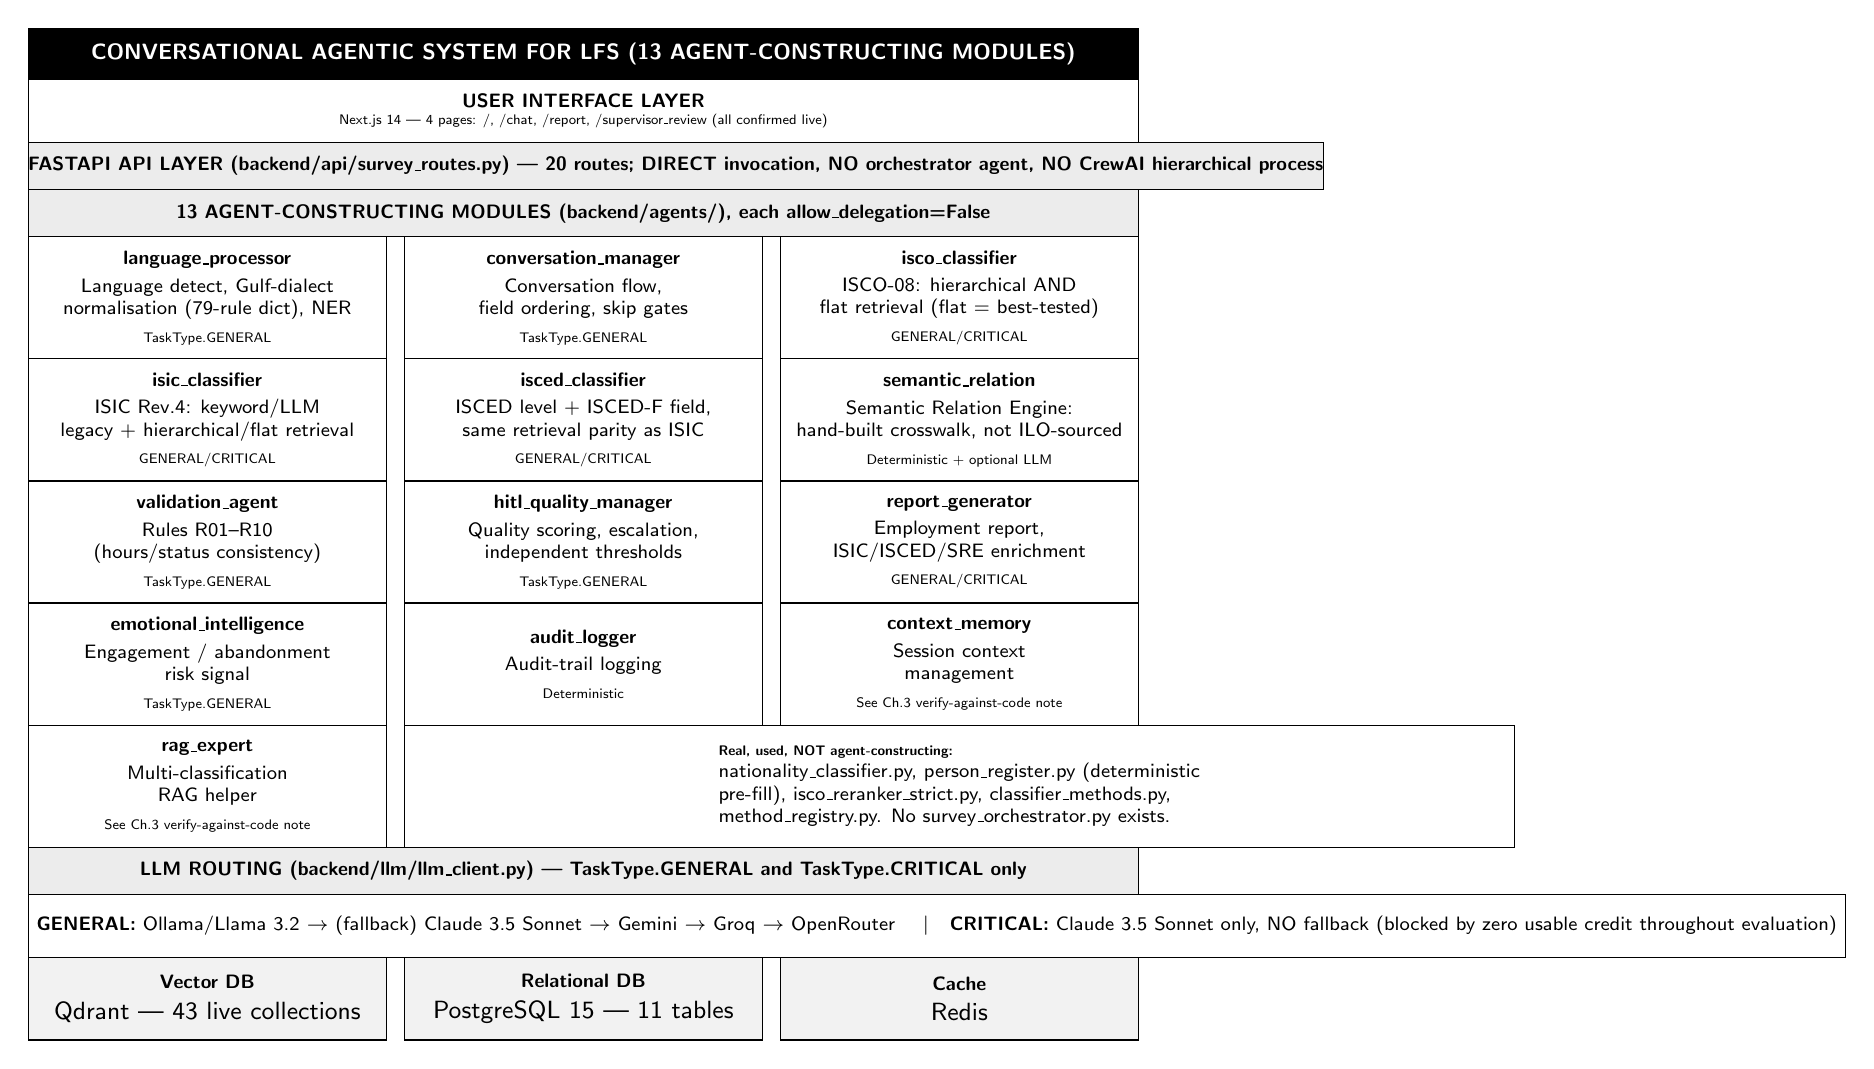
\begin{tikzpicture}[every node/.style={outer sep=0pt}]

\def\xL{2.275}
\def\xM{7.050}
\def\xR{11.825}

%% Title
\node[titlebar, anchor=north west] at (0, 0)
  {CONVERSATIONAL AGENTIC SYSTEM FOR LFS (13 AGENT-CONSTRUCTING MODULES)};

%% UI Layer
\node[fullbar, anchor=north west] at (0, -0.65cm)
  {\textbf{USER INTERFACE LAYER}\\[-2pt]
   {\tiny Next.js~14 --- 4 pages: /, /chat, /report, /supervisor\_review (all confirmed live)}};

%% API layer -- no orchestrator agent, no hierarchical process
\node[shadebar, anchor=north west] at (0, -1.45cm)
  {FASTAPI API LAYER (backend/api/survey\_routes.py) --- 20 routes; DIRECT invocation, NO orchestrator agent, NO CrewAI hierarchical process};

%% Specialist agents header
\node[shadebar, anchor=north west] at (0, -2.05cm)
  {13 AGENT-CONSTRUCTING MODULES (backend/agents/), each allow\_delegation=False};

%% Row 1: 3 modules
\node[agentcell, anchor=north west] at (0, -2.65cm)
  {\textbf{language\_processor}\\[2pt]
   Language detect, Gulf-dialect\\normalisation (79-rule dict), NER\\[2pt]
   {\tiny TaskType.GENERAL}};

\node[agentcell, anchor=north west] at (4.775cm, -2.65cm)
  {\textbf{conversation\_manager}\\[2pt]
   Conversation flow,\\field ordering, skip gates\\[2pt]
   {\tiny TaskType.GENERAL}};

\node[agentcell, anchor=north west] at (9.55cm, -2.65cm)
  {\textbf{isco\_classifier}\\[2pt]
   ISCO-08: hierarchical AND\\flat retrieval (flat = best-tested)\\[2pt]
   {\tiny GENERAL/CRITICAL}};

%% Row 2: 3 modules
\node[agentcell, anchor=north west] at (0, -4.20cm)
  {\textbf{isic\_classifier}\\[2pt]
   ISIC Rev.4: keyword/LLM\\legacy + hierarchical/flat retrieval\\[2pt]
   {\tiny GENERAL/CRITICAL}};

\node[agentcell, anchor=north west] at (4.775cm, -4.20cm)
  {\textbf{isced\_classifier}\\[2pt]
   ISCED level + ISCED-F field,\\same retrieval parity as ISIC\\[2pt]
   {\tiny GENERAL/CRITICAL}};

\node[agentcell, anchor=north west] at (9.55cm, -4.20cm)
  {\textbf{semantic\_relation}\\[2pt]
   Semantic Relation Engine:\\hand-built crosswalk, not ILO-sourced\\[2pt]
   {\tiny Deterministic + optional LLM}};

%% Row 3: 3 modules
\node[agentcell, anchor=north west] at (0, -5.75cm)
  {\textbf{validation\_agent}\\[2pt]
   Rules R01--R10\\(hours/status consistency)\\[2pt]
   {\tiny TaskType.GENERAL}};

\node[agentcell, anchor=north west] at (4.775cm, -5.75cm)
  {\textbf{hitl\_quality\_manager}\\[2pt]
   Quality scoring, escalation,\\independent thresholds\\[2pt]
   {\tiny TaskType.GENERAL}};

\node[agentcell, anchor=north west] at (9.55cm, -5.75cm)
  {\textbf{report\_generator}\\[2pt]
   Employment report,\\ISIC/ISCED/SRE enrichment\\[2pt]
   {\tiny GENERAL/CRITICAL}};

%% Row 4: 3 modules
\node[agentcell, anchor=north west] at (0, -7.30cm)
  {\textbf{emotional\_intelligence}\\[2pt]
   Engagement / abandonment\\risk signal\\[2pt]
   {\tiny TaskType.GENERAL}};

\node[agentcell, anchor=north west] at (4.775cm, -7.30cm)
  {\textbf{audit\_logger}\\[2pt]
   Audit-trail logging\\[2pt]
   {\tiny Deterministic}};

\node[agentcell, anchor=north west] at (9.55cm, -7.30cm)
  {\textbf{context\_memory}\\[2pt]
   Session context\\management\\[2pt]
   {\tiny See Ch.3 verify-against-code note}};

%% Row 5: 1 module + note
\node[agentcell, anchor=north west] at (0, -8.85cm)
  {\textbf{rag\_expert}\\[2pt]
   Multi-classification\\RAG helper\\[2pt]
   {\tiny See Ch.3 verify-against-code note}};

\node[fullbar, anchor=north west, minimum height=1.55cm, align=left] at (4.775cm, -8.85cm)
  {\tiny \textbf{Real, used, NOT agent-constructing:}\\
   nationality\_classifier.py, person\_register.py (deterministic\\
   pre-fill), isco\_reranker\_strict.py, classifier\_methods.py,\\
   method\_registry.py. No survey\_orchestrator.py exists.};

%% LLM tiers -- real
\node[shadebar, anchor=north west] at (0, -10.40cm)
  {LLM ROUTING (backend/llm/llm\_client.py) --- TaskType.GENERAL and TaskType.CRITICAL only};

\node[fullbar, anchor=north west] at (0, -11.00cm)
  {\textbf{GENERAL:} Ollama/Llama~3.2 $\to$ (fallback) Claude~3.5~Sonnet $\to$ Gemini $\to$ Groq $\to$ OpenRouter
   \quad\textbar\quad
   \textbf{CRITICAL:} Claude~3.5~Sonnet only, NO fallback (blocked by zero usable credit throughout evaluation)};

%% Storage row -- verified only
\node[dbcell, anchor=north west] at (0, -11.80cm)
  {\textbf{Vector DB}\\[3pt]
   {\small Qdrant --- 43 live collections}};

\node[dbcell, anchor=north west] at (4.775cm, -11.80cm)
  {\textbf{Relational DB}\\[3pt]
   {\small PostgreSQL 15 --- 11 tables}};

\node[dbcell, anchor=north west] at (9.55cm, -11.80cm)
  {\textbf{Cache}\\[3pt]
   {\small Redis}};

\end{tikzpicture}

\caption{System architecture, corrected against the live implementation:
13 real agent-constructing modules, direct API-layer orchestration (no
CrewAI hierarchical process), and the real two-tier LLM routing design.}
\label{fig:system-architecture}
\end{figure}

% arch_diagram.tex was rebuilt 2026-08-29: the original depicted 10
% numbered agents, a false "Hierarchical Process" label, and LLM
% providers (GPT-4o, Llama 3.1 70B) unused anywhere in this project. It
% now shows the real 13 modules, the real GENERAL/CRITICAL LLM tiers, and
% no hierarchical-delegation claim.

\section{Agent Module Specification}
\label{sec:arch-agents}
% ------------------------------------------------------------

Table~\ref{tab:ch3-agents} lists the 13 real \texttt{crewai.Agent}-constructing
modules. Responsibilities are stated at the level this thesis can verify
directly from module names and CLAUDE.md's own module-by-module audit;
per-module internal implementation detail beyond what is cited elsewhere in
this chapter should be checked against the live source before being cited
further in this thesis.

\begingroup
\setlength{\tabcolsep}{4pt}
\footnotesize
\renewcommand{\arraystretch}{1.5}
\begin{longtable}{>{\raggedright}p{3.5cm}
                  >{\raggedright}p{7.0cm}
                  >{\raggedright\arraybackslash}p{3.0cm}}
\caption{The 13 real CrewAI-agent-constructing modules under \texttt{backend/agents/}.}
\label{tab:ch3-agents}\\
\toprule
\textbf{Module} & \textbf{Role} & \textbf{LLM Tier} \\
\midrule
\endfirsthead
\multicolumn{3}{c}{\tablename\ \thetable{} -- \textit{continued}} \\
\toprule
\textbf{Module} & \textbf{Role} & \textbf{LLM Tier} \\
\midrule
\endhead
\bottomrule
\endlastfoot
\texttt{language\_processor} & Language detection, Gulf-dialect normalisation
  (79-rule dictionary), code-switch detection, NER & GENERAL \\
\texttt{conversation\_manager} & Conversation FSM; field ordering; skip-gate
  evaluation & GENERAL \\
\texttt{isco\_classifier} & ISCO-08 classification: hierarchical and flat
  retrieval, keyword fallback, optional LLM rerank & GENERAL/CRITICAL per
  call site \\
\texttt{isic\_classifier} & ISIC Rev.~4 classification: keyword/LLM legacy
  pipeline plus hierarchical and flat retrieval paths & GENERAL/CRITICAL \\
\texttt{isced\_classifier} & ISCED level (keyword) + ISCED-F field
  (keyword, plus hierarchical/flat retrieval) & GENERAL/CRITICAL \\
\texttt{validation\_agent} & Rules R01--R10 (Section~\ref{sec:arch-principles})
  plus an optional Stage-2 LLM semantic check & GENERAL \\
\texttt{hitl\_quality\_manager} & Quality scoring and escalation to
  \texttt{hitl\_queue}, independent thresholds from \texttt{ISCOClassifier} & GENERAL \\
\texttt{audit\_logger} & Audit-trail logging & (module constructs an Agent;
  logging logic itself is deterministic) \\
\texttt{report\_generator} & Employment report generation, ISIC/ISCED/SRE
  enrichment persistence & GENERAL/CRITICAL \\
\texttt{emotional\_intelligence} & Engagement/abandonment-risk signal & GENERAL \\
\texttt{semantic\_relation} & The Semantic Relation Engine
  (Section~\ref{sec:arch-sre}) & Deterministic core; optional LLM
  re-inference path exists \\
\texttt{context\_memory} & Redis-backed session state (24h TTL); tracks
  which required LFS fields are still missing so
  \texttt{ConversationManager} avoids duplicate questions --- confirmed
  directly from the module's own docstring & -- \\
\texttt{rag\_expert} & A \emph{second}, distinct hierarchical ISCO-08
  retrieval mechanism from \texttt{isco\_classifier}'s own beam search:
  broad e5-small semantic search, then parent-code expansion (adding each
  candidate's sub-major/major ancestors) --- confirmed directly from the
  module's own docstring; not independently benchmarked against
  \texttt{isco\_classifier}'s pipelines in this thesis & -- \\
\end{longtable}
\endgroup

Not agent-constructing, but real and used: \texttt{nationality\_classifier.py},
\texttt{person\_register.py} (deterministic pre-fill from the
\texttt{person\_register} table), \texttt{isco\_reranker\_strict.py},
\texttt{classifier\_methods.py} (shared constants), and
\texttt{method\_registry.py} (introspection utility).

% ------------------------------------------------------------
\section{Conversation Flow}
\label{sec:arch-fsm}
% ------------------------------------------------------------

\textbf{Verified directly against \texttt{backend/agents/conversation\_
manager.py}'s own module docstring (not restated from an earlier draft).}
The system is a UAE Labour Force Survey implementation with a real
five-state FSM --- \texttt{GREETING}, \texttt{COLLECTING\_INFO},
\texttt{CLARIFYING}, \texttt{VALIDATING}, \texttt{COMPLETING}, confirmed as
an actual \texttt{ConversationState} enum in the live code. The
\texttt{\_get\_field\_order(collected\_data)} method is recomputed after
every turn, enabling real-time path switching.

\textbf{Real field list, all three paths}, confirmed directly:

\begin{itemize}
  \item \textbf{All paths} (16 fields): \texttt{employment\_status} (C1),
  \texttt{education\_level} (B5), \texttt{gender} (B1),
  \texttt{nationality} (B3), \texttt{marital\_status} (B4),
  \texttt{emirate} (B8), \texttt{uae\_residence\_duration} (B9),
  \texttt{vocational\_training} (B7), \texttt{main\_skills} (H1),
  \texttt{training\_participation} (H3),
  \texttt{labour\_market\_barriers} (H5), \texttt{platform\_work} (I1),
  \texttt{online\_business} (I4), \texttt{question\_clarity} (K1),
  \texttt{ai\_preference} (K3), \texttt{data\_confidence} (K4).
  \item \textbf{Employed path} adds 18 fields, including
  \texttt{contract\_type} (D7, gated on \texttt{employment\_nature ==
  paid\_employee}) and \textbf{\texttt{monthly\_wage\_range} (E1, gated on
  \texttt{employment\_nature == paid\_employee})}.
  \item \textbf{Unemployed path} adds \texttt{job\_search\_active} (F1),
  \texttt{job\_search\_methods} (F2, gated on F1~=~yes), and
  \textbf{\texttt{available\_for\_work} (F3) --- if F1~=~no AND F3~=~no,
  the respondent is reclassified to \texttt{not\_in\_labour\_force}} ---
  plus \texttt{unemployment\_duration} (F4), \texttt{desired\_job\_type}
  (F5), \texttt{ever\_worked} (F7), and, if ever worked,
  \texttt{last\_job\_title} (G1) and \texttt{reason\_left\_job} (G3).
  \item \textbf{Outside-labour-force path} adds \texttt{outside\_lf\_reason}
  (F6), \texttt{ever\_worked} (F7), and \texttt{last\_job\_title} (G1) if
  ever worked.
\end{itemize}

At least one further real, conditional field exists beyond this docstring
summary: \texttt{field\_of\_study} (B6), applying to all three paths but
gated on \texttt{education\_level >= bachelor}, feeding the ISCED-F
classifier (Appendix~\ref{app:questionnaire}). The list above is real and
directly sourced, but should not be assumed exhaustive of every
conditional field without reading the function bodies beyond the module
docstring.

\textbf{This is a real, important correction to Section~\ref{sec:arch-principles}
above and to Chapter~\ref{chap:implementation}}: the E1 wage gate and the
F3 not-in-labour-force re-routing rule \emph{do} exist in this codebase,
exactly as an earlier internal draft of this thesis described --- what was
wrong in that draft was attributing them to \texttt{ValidationAgent}'s
R01--R10 rule set specifically. They are real, but they live in
\texttt{ConversationManager} as FSM skip-gate/field-relabelling logic, a
different mechanism from the ten deterministic consistency rules
(Section~\ref{sec:arch-principles}). Both are real; they are simply two
different things that an earlier draft had conflated into one.

%% VERIFY AGAINST CODE: the full skip-gate count (an earlier draft claimed
%% "11 skip gates" total) was not exhaustively re-counted against every
%% conditional in conversation_manager.py in this pass -- the module
%% docstring above documents at least 6 explicit "if X" gates (D7, E1, F2,
%% F3, G1 x2, G3); a complete count would require reading the function
%% bodies beyond the docstring summary. Frontend component names and exact
%% quick-reply-field counts remain unverified -- check frontend/ directly.

% ------------------------------------------------------------
\section{ISCO-08 Retrieval Pipelines}
\label{sec:arch-rag}
% ------------------------------------------------------------

Two retrieval configurations were implemented and empirically compared, not
one assumed to be superior.

\textbf{Hierarchical retrieval.} A four-stage, parent-filtered beam search
(major $\to$ sub-major $\to$ minor $\to$ unit group) built on a generic
\texttt{HierarchyBeamSearchEngine}, with weighted confidence
$c = 0.10s_1 + 0.20s_2 + 0.20s_3 + 0.50s_4$ across the four stage
similarities.

\textbf{Flat retrieval.} A single-collection direct search over the
unit-group level only, with full ancestry (major/sub-major/minor)
reconstructed via a lookup table rather than traversed live.

\textbf{The catalogue itself.} 436 unit groups, matching the official
ISCO-08 structure exactly --- corrected via a direct cross-check against the
primary ILO source, resolving 19 non-standard codes, 14 missing codes, and 6
further mislabelled codes an earlier, WISCO-only comparison could not catch.
One disclosed exception remains: Major Group~0 (Armed Forces) uses
non-standard 4-digit codes (\texttt{"0110"} etc.) instead of ISCO-08's own
3-digit convention, kept for compatibility with the rest of this codebase's
4-digit assumptions rather than fixed unilaterally.

\textbf{The empirical result (full detail in Chapter~\ref{chap:results}):}
on a real, external, 18,747-case benchmark (WISCO), \textbf{flat retrieval
outperformed hierarchical retrieval by 10.84 percentage points}
(21.19\% vs.\ 10.35\%, McNemar $p \approx 1.86\times10^{-301}$) --- the
opposite of what the four-stage design in the original draft of this thesis
assumed and reported. This is stated here as a real, tested finding, and
the best-tested configuration actually used for this thesis's headline
ISCO-08 result (Chapter~\ref{chap:results}) is flat retrieval, not
hierarchical.

\textbf{HNSW indexing: no custom parameters are actually set.} An earlier
internal draft of this thesis claimed specific tuned values (M=32,
ef\_construct=256); a direct search of \texttt{backend/rag/} found no
\texttt{HnswConfig} usage anywhere --- collections are created with plain
\texttt{VectorParams}/\texttt{Distance} only, meaning Qdrant's untouched
defaults are used. This is a real correction, not an unverified gap: the
original draft's specific tuned values do not exist in this codebase.
\textbf{Two further original-draft claims confirmed real}, checked
directly: the ``head chef'' keyword-pre-filter example is exact ---
\texttt{\_keyword\_major\_hint()} in \texttt{isco\_classifier.py} maps
\texttt{"head chef"} (and \texttt{"sous chef"}, \texttt{"executive chef"})
to major group \texttt{"5"} (Service and Sales Workers) by name, verbatim.
Synonym enrichment is also real, in the legacy catalogue builder
(\texttt{\_UNIT\_SYNONYMS} in \texttt{load\_full\_isco.py}), with the
module's own comment giving essentially the same example: ``chef''
$\to$ 5120 Cooks, not 2151.
%% VERIFY AGAINST CODE: the original draft's specific "8,720+ chunks" and
%% "50+ synonyms" counts were not independently re-counted in this pass.

% ------------------------------------------------------------
\section{ISIC Rev.~4 Industry Classifier}
\label{sec:arch-isic}
% ------------------------------------------------------------

\texttt{ISICClassifier} implements the full ISIC Rev.~4 hierarchy (Section
$\to$ Division $\to$ Group $\to$ 4-digit Class) via a legacy keyword/LLM
pipeline, plus real, live hierarchical- and flat-retrieval paths built at
architectural parity with the ISCO-08 pipeline, including the same
official-text enrichment and \texttt{multilingual-e5-large} embedding for
the flat path specifically. The live-indexed catalogue currently covers
\textbf{134 of 419} official ISIC Rev.~4 4-digit classes --- stated exactly,
not as ``100+'' --- with 13 further codes in the underlying keyword table
found not to correspond to any real official ISIC code (disclosed, not yet
individually corrected; excluded specifically from the enriched flat
collection after a live-tested regression showed keeping them caused
active misclassification).

Representative mappings (matching this project's own live-verified test
queries):
\begin{itemize}
  \item ``I build mobile apps at a software company'' $\to$ ISIC 6201
  (Computer programming activities)
  \item ``construction labourer on a residential building site'' $\to$
  ISIC 4100 (Construction of buildings)
\end{itemize}

% ------------------------------------------------------------
\section{ISCED Classifier}
\label{sec:arch-isced}
% ------------------------------------------------------------

\texttt{ISCEDClassifier} produces two independently-scored dimensions:
ISCED~2011 attainment level (0--8) and ISCED-F~2013 field of specialisation,
combined as $\text{confidence} = 0.4 \times \text{level\_conf} + 0.6 \times
\text{field\_conf}$ --- confirmed directly against the live
\texttt{isced\_classifier.py} source (line 609).
The ISCED-F live-indexed catalogue covers \textbf{63 of approximately 80}
detailed fields, with hierarchical and flat retrieval paths built at the
same parity as ISIC Rev.~4 (2 further non-standard codes disclosed and
excluded from the enriched flat collection, same rationale as ISIC).

Example: ``Bachelor's degree in computer science'' correctly retrieves
ISCED-F 0613 (Software and applications development and analysis) via the
flat-retrieval path, live-verified.

% ------------------------------------------------------------
\section{Semantic Relation Engine}
\label{sec:arch-sre}
% ------------------------------------------------------------

The Semantic Relation Engine (\texttt{backend/agents/semantic\_relation.py})
cross-validates ISCO-08, ISIC Rev.~4, and ISCED/ISCED-F classifications.
\textbf{The crosswalk tables are hand-built}, not sourced from an official
ILO or UNESCO correspondence document --- this project searched the
complete, official 433-page ISCO-08 Volume~I document page-by-page and
confirmed no ISCO-08$\leftrightarrow$ISIC correspondence table exists in
it, nor in any other ILO document found. This is disclosed here as a
limitation (further discussed in Chapter~\ref{chap:conclusion}), not
presented as sourced from an official table.

\textbf{The real scoring formula}, taken directly from the live
\texttt{analyse()} method (starting at line 340 of the source file, verified
2026-08-24):

\begin{equation}
\text{raw\_score} =
\begin{cases}
0.55\,\text{score}_{\text{ISIC}} + 0.45\,\text{score}_{\text{ISCED}} &
  \text{both ISIC and ISCED data present} \\
\text{score}_{\text{ISIC}} & \text{ISIC only} \\
\text{score}_{\text{ISCED}} & \text{ISCED only} \\
0.80 & \text{neither present (assume plausible)}
\end{cases}
\end{equation}

A partial-credit step then softens the raw score for each MODERATE-severity
violation found: $\text{raw\_score} \mathrel{+}= 0.15 \times
n_{\text{moderate}} \times (1 - \text{raw\_score})$, clipped to $[0,1]$.
The final \texttt{score} is this value rounded to 4 decimal places, with
$\text{is\_coherent} = (\text{score} \geq 0.70)$.

\textbf{This corrects the original draft in two ways}, both confirmed
against the live code: (1) the partial-credit step above was previously
omitted entirely; and (2) violation \textbf{severity} (LOW/MODERATE/HIGH)
is a genuinely \emph{separate}, gap-based mechanism, not derived from the
coherence-score bands --- it is computed from how many ISCED levels a
respondent's level falls outside the ISCO major group's expected
$[\text{min}, \text{max}]$ range: gap~$\leq 1 \to$ LOW, gap~$=2 \to$
MODERATE, gap~$>2 \to$ HIGH. A separate, independent confidence-adjustment
band applies to the \emph{caller's} confidence based on the coherence
\texttt{score} itself: $\geq 0.90 \to +0.10$; $\geq 0.70 \to +0.05$;
$\geq 0.50 \to -0.05$; else $\to -0.20$. The original draft's single
severity/confidence table conflated these two genuinely different
mechanisms into one, which this correction separates.

Sub-major-group strict rules (e.g.\ Health Professionals requiring ISIC
section~Q and ISCED~$\geq 7$; ICT Professionals preferring ISIC section~J;
Chief Executives requiring ISCED~$\geq 6$) are confirmed present but
confirmed still hand-built, not rebuilt from an official correspondence
source --- this remains real, open work (Chapter~\ref{chap:conclusion}).

A HIGH-severity SRE result genuinely escalates to the live HITL queue,
verified three times against the real
\texttt{/survey/sessions/\{id\}/message} endpoint: 100\% of 15 HIGH-severity
cases escalated, 0\% of 46 non-HIGH cases did, identically across all three
runs.

% ------------------------------------------------------------
\section{Technology Stack}
\label{sec:arch-stack}
% ------------------------------------------------------------

\begin{table}[htbp]
\centering
\caption{Technology stack, versions verified against \texttt{requirements.txt}.}
\label{tab:ch3-stack}
\footnotesize\renewcommand{\arraystretch}{1.4}
\resizebox{\textwidth}{!}{%
\begin{tabular}{>{\raggedright}p{2.6cm}
                >{\raggedright}p{5.0cm}
                >{\raggedright\arraybackslash}p{4.6cm}}
\toprule
\textbf{Layer} & \textbf{Technology} & \textbf{Note} \\
\midrule
Backend & FastAPI 0.131.0, SQLAlchemy 2.0.46, Alembic 1.18.4 &
  \\
AI Orchestration & CrewAI 1.9.3 &
  13 agent-constructing modules; no hierarchical delegation \\
Vector DB & Qdrant client 1.17.0 &
  Multiple coexisting collection profiles, not a fixed set of four \\
Embeddings & \texttt{intfloat/multilingual-e5-small} (production default,
  384-dim); \texttt{-e5-large} (1024-dim) additive profile, measurably more
  accurate, not yet switched to default & \\
Database & PostgreSQL 15, 11 tables & \\
Cache & Redis (client 7.2.0) & \\
General LLM & Ollama/Llama~3.2, temp~0.3, with real fallback chain & \\
Critical LLM & Claude~3.5~Sonnet, temp~0.0, no fallback by design &
  Blocked by zero usable credit throughout this project's evaluation history \\
Deployment & Docker Compose & \\
\bottomrule
\end{tabular}
}
\end{table}

% ------------------------------------------------------------
\section{End-to-End Data Flow}
\label{sec:arch-dataflow}
% ------------------------------------------------------------

A survey turn flows, at a level confirmed by this project's own real
end-to-end login-through-session test (Chapter~\ref{chap:evaluation}):
authentication (OTP $\to$ JWT) $\to$ session creation with Person Register
pre-fill $\to$ per-turn language processing, field advancement, and
classification (ISCO/ISIC/ISCED as applicable) $\to$ Semantic Relation
Engine scoring once all three are available $\to$ validation-rule checking
$\to$ HITL escalation if warranted $\to$ decision logging $\to$ response.
%% VERIFY AGAINST CODE: the original draft's specific lettered sub-steps
%% (a)-(l) were not independently re-verified line-by-line against
%% survey_routes.py in this pass; the sequence above is stated at the
%% level this project's real orchestration-correctness test suite
%% (test_orchestration_correctness.py) actually asserts.
